\section{Sortering og søking}

\subsection{Sortering}

\subsubsection{Stabilitet}

\subsubsection{Sammenligningsbaserte sorteringsalgoritmer}

\noindent \textbf{Merge sort}\\
Merge-sort deler listen i to helt til den har en stor samling med lister som har bare ett element. Dermed har man en samling av sorterte lister. Disse slås så sammen ved å sammenligne det første elementet i to lister. Den minste legges fremst i en ny liste, og fjernes fra den opprinnelige listen. Dette gjøres for hver liste rekursivt, som til slutt gir en sortert liste med alle elementene.
\\\\
Merge-sort er en “splitt-og-hersk” algoritme. Merge-sort er effektiv. Deler opp problemet i stadig mindre biter, og når bitene er små nok flettes de sammen i sortert rekkefølge.

\begin{lstlisting}
    function MERGE-SORT(A,p,r)
    	if p < r then
    		q = $\left \lceil{(p + r)/2}\right \rceil$
    		MERGE-SORT(A,p,r)
    		MERGE-SORT(A,q + 1,r)
    		MERGE(A,p,q,r)
    	end if
    end function
\end{lstlisting}

\begin{lstlisting}
    function MERGE(A,p,q,r)
	    n1 = q - pr + 1
    	n2 = r - q
	    let L[1...n1 + 1] and R[1...n2 + 1] be new arrays
        for i = 1 to n1 do
	        L[i] = A[p + i - 1]
        end for
        for j = 1 to n2 do
        	R[j] = A[q + j]
        end for
        L[[n1] + 1] = $\infty$
        r[[n2] + 1] = $\infty$
        i = 1
        j = 1
        for k = p to r do
        	if L[i] $\leq$ R[j] then
        		A[k] = L[i]
        		i = i + 1
        	else
        		if A[k] = R[j] then
        			j = j + 1
        		end if
        	end if
        end for
        end function
\end{lstlisting}

\noindent \textbf{Eksempel}\\
Gitt tallfølgen 6, 5, 3, 1, 8, 7, 2, 4. Tallene deles opp i to grupper, 6, 5, 3, 1 og 8, 7, 2, 4. Disse deles så opp i to igjen; 6, 5 og 3, 1 og 8, 7 og 2, 4. Disse deles så opp i ett og ett tall. Sorteres så etter rekkefølge innad i toergruppene. Har da; 5, 6 og 1, 3 og 7, 8 og 2, 4. Slår så sammen to og to grupper til to grupper på fire, sortert: 1, 3, 5, 6 og 2, 4, 7, 8. Slår til slutt sammen de to firergruppene, sortert: 1, 2, 3, 4, 5, 6, 7, 8.

\begin{figure}[H]
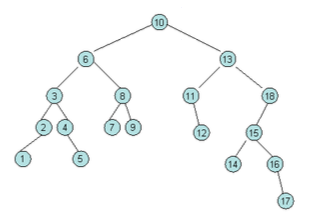
\includegraphics[scale=0.7]{images/mergesort}
\centering %centering the image
\caption{Merge sort}
\label{fig:mergesort}
\end{figure}

\noindent \textbf{Quicksort}\\
Quicksort er enda en “splitt-og-hersk”-algoritme. Man starter gjerne Quicksort ved å randomisere listen. Den starter med å velge et pivotelement. Den deler deretter listen i to partisjoner: en med elementene som er mindre eller lik pivoten, og en med elementene som er større enn pivot. Deretter kaller den seg selv rekursivt på de to partisjonene. Deretter fletter man sammen de to partisjonene.

\begin{lstlisting}
    function QUICKSORT(A,p,r)
    	if p < r then
    		q = PARTITION(A,p,r)
    		QUICKSORT(A,p,q - 1)
    		QUICKSORT(A.q + 1, r)
    	end if
    end function
\end{lstlisting}

\begin{lstlisting}
    function PARTITION(A,p,r)
	    x = A[r]
    	i = p - 1
    	for j = p to r - 1 do
    		if A[j] $\leq$ x then
    			i = i + 1
    			exchange A[i] with A[j]
    		end if
    	end for
    	exchange A[i + 1] with A[j]
    	return i + 1
    end function
\end{lstlisting}

\noindent \textbf{Bubblesort}\\
Bubblesort tester to og to naboelementer. Dersom den første er større bytter de plass. Effektiv på små datamengder. Denne algoritmen bruker sammenligning.

\begin{lstlisting}
    for i = 0 to A.length - 1 do
    	for j = A.length downto i + 1 do
		    if A[j] < A[j - 1] then
		    	exchange A[j] with A[j - 1]
		    end if
	    end for
    end for
\end{lstlisting}

\noindent \textbf{Eksempel}\\
Gitt tallfølgen 6, 5, 3, 1, 8, 7, 2 4. Vil sorteres slik at etter en runde vil rekken bli 5, 3, 1, 6, 7, 2, 4, 8. Neste runde vil den være: 3, 1, 5, 6, 2, 4, 7, 8. Så vil den bli: 1, 3, 5, 2, 4, 6, 7, 8. Deretter: 1, 3, 2, 4, 5, 6, 7, 8. Etter fem runder blir rekkefølgen: 1, 2, 3, 4, 5, 6, 7, 8.\\

\noindent \textbf{Insertion sort}\\
Insertion-sort minner litt om selection-sort. Man tar det første usorterte elementet $x$, og sammenligner det med de sorterte elementene. Hvis man når et element som er mindre enn $x$ stopper man man gjennomgangen, og tar for seg neste $x$. Dette fungerer på samme måte som de fleste sorterer en korthånd.
\\\\
Insertion-sort er en enkel sorteringsalgoritme. Den tar de to første elementene og plasserer i forhold til hverandre. Deretter plasserer den det neste i forhold til de to forrige, osv. Veldig effektiv å bruke på små mengder. Kan f.eks. brukes i slutten på en Quick-sort algoritme.

\begin{lstlisting}
    for j = 0 to A.length do
	    key = A[j]
	    i = j - 1
	    while i > 0 and A[i] > key do
	    	A[i + 1] = A[1]
	    	i = i - 1
	    end while
	    A[i] + 1 = key
    end for
\end{lstlisting}

\noindent \textbf{Eksempel}\\
Gitt tallrekken 6, 5, 3, 1, 8, 7, 2, 4. Begynner med 6, som er første tall. Ser så på 5. 5 er mindre enn 6, og flyttes til plass null. Rekken ser da slik ut: 5, 6, 3, 1, 8, 7, 2, 4. Ser så på plass nummer to, tallet 3. Det er mindre enn både 5 og 6, og flyttes først. Tallrekken er da: 3, 5, 6, 1, 8, 7, 2, 4. Plass tre er 1. Det er minst av alle, og settes ført. Da er tallrekken: 1, 3, 5, 6, 8, 7, 2, 4. Plass nummer fire er tallet 8. Det er større enn alle tidligere tall, og blir stående. Plass fem er 7. Det er mindre enn 8 og flyttes til plass fire: 1, 3, 5, 6, 7, 8, 2, 4. Plass seks er 2, som er mindre enn nesten alle. Flyttes til plass en, og tallrekken blir: 1, 2, 3, 5, 6, 7, 8, 4. Da er det bare 4 igjen, som er mindre enn mange av tallene, og plasseres rett i plass tre. Da er tallfølgen ferdig sortert: 1, 2, 3, 4, 5, 6, 7, 8.\\

\noindent \textbf{Selection sort}\\

\subsubsection{Andre sorteringsalgoritmer}

\noindent \textbf{Heapsort}\\
Heapsort benytter seg av en heap som datastruktur. Lager en heap av alle elementene slik at hver node sine barn er mindre enn den selv. Det øverste elementet er alltid det største. Deretter plukkes det øverste elementet ut, for så å sortere heapen igjen, og ta ut det øverste elementet igjen. Fortsetter til heapen er tom.

\begin{lstlisting}
    BUILDMAXHEAP(A)
        for i = A.length downto 2 do
	        exchange A[1] with A[i]
	        A.heapSize = A.heapSize - 1
	        MAX-HEAPIFY(A,1)
        end for
\end{lstlisting}

\noindent \textbf{Counting sort}\\
Counting-sort tar et heltall $N$ mellom $0$ og $k$. Lager en liste med verdier fra $0$ til $k$ og setter inn tallene på sin plass i listen. Fungerer best når verdiene på tallene som sorteres ligger tett etterhverandre og $k$ ikke er for høy.

\begin{lstlisting}
    function COUNTINGSORT(A,B,k)
	    let C[0...k] be a new array
    	for i = 0 to k do
    		C[i] = 0
    	end for
    	for j = 1 to A.length do
    		C[A[j]] = C[A[j]] + 1
    	end for
    	for i = 0 to k do
    		C[i] = C[i] + C[i - 1]
    	end for
    	for j = A-length downto 1 do
    		B[C[A[j]]] = A[j]
    		C[A[j]] = C[A[j]] - 1
    	end for
    end function
\end{lstlisting}

\noindent Har kjøretid $O(n)$ i verste tilfelle, dersom $k = O(n)$ og $d = O(1)$.\\

\noindent \textbf{Eksempel}\\
Gitt A = [3, 3, 1, 4, 4, 3, 1, 2, 3, 5]. Hvordan ser C[0...6] ut idet Counting-Sort(A, B, 6) returnerer?
\\\\
[0, 0, 2, 3, 7, 9, 10] Tellesortering teller først forekomster, gjør så tellingene kumulative, og så dekrementerer disse under innsetting. Så tellingene til slutt tilsvarer altså hvor mange som er strengt mindre. F.eks. vil C[3] hvor mange verdier som er mindre enn 3. Her gis også enkelte andre svar noe uttelling. \\

\noindent \textbf{Radix sort}\\
Radix-sort sorterer tall i et gitt tallsystem (her titallsystemet) etter minste signifikante siffer.

\begin{lstlisting}
    function RADIXSORT(A,d)
    	for i = 1 to d do
    		Bruk Stabble sort til å sortere array A
    	end for
    end function
\end{lstlisting}

\noindent \textbf{Bucketsort}\\
Veldig lik Counting-sort, men bruker såkalte “bøtter” man putter tallene i. For eksempel [5,6) betyr at verdier større eller lik 5, men mindre enn 4 skal i bøtten.

\begin{lstlisting}
    function BUCKETSORT(A)
	    n = A.length
	    la B[0...n - 1] være et nytt array
	    for i = 0 to n - 1 do
	    	Gjør B[i] til en tom liste
	    end for
	    for i = 1 to n do
    		Sett inn A[i] i lista B[⌊nA[i]⌋]
    	end for
	    for i = 0 to n - 1 do
		    Sorter lista B[i] med INSERTIONSORT(B[i])
	    end for
	    Konkatiner listene B[0], B[1], …, B[n - 1] i rekkefølge
    end function
\end{lstlisting}

\noindent Bucket-Sort endrer kjøretid fra beste til verste tilfelle, og bruker ikke sammenligning.
\\\\
\noindent \textbf{Eksempel}\\
Lager bøtter for tallintervallene. Gitt tallene 29, 25, 3, 49, 9, 37, 21, 43. Lager bøtter for 0-9, her havner 3 og 9. 10-19 er tom. 20-29 år 21, 25 og 29. 30-39 får 37. 40-49 får 43 og 49.

\begin{figure}[H]
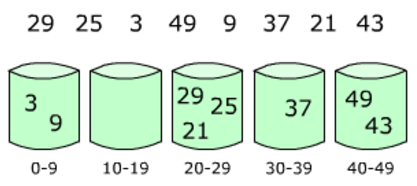
\includegraphics[scale=0.5]{images/bucketsort1}
\centering %centering the image
\caption{Bucketsort første trinn}
\label{fig:bucketsort1}
\end{figure}

\noindent Når dette så skal setter sammen til en sortert tallfølge hentes tallene opp fra bøttene igjen.

\begin{figure}[H]
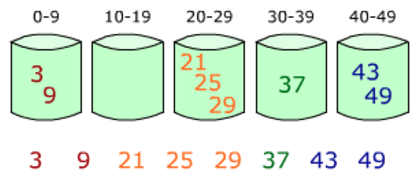
\includegraphics[scale=0.5]{images/bucketsort2}
\centering %centering the image
\caption{Bucketsort andre trinn}
\label{fig:bucketsort2}
\end{figure}

\noindent Tallfølgen blir da til slutt 3,9, 21, 25, 29, 37, 43, 49.\\

\noindent \textbf{Topologisk sortering}\\
Topologisk sortering bruker en DAG til å finne en rekkefølge gjennom alle elementene i grafen. Det tillates ikke sykler. Man begynner i noden som ikke har noen kanter inn til seg.

\begin{lstlisting}
    function TOPOLOGICALSORT(G)
    	DFS(G) to compute finish times v.f for each vertex v.
    	as each vertex is finished, insert it onto the end of the list
    	return the list of vertices
    end function

\end{lstlisting}


\subsection{Søking}

\subsubsection{Brute force}

\subsubsection{Binærsøk}
Et binært søketre er et tre som tilfredsstiller binært-søketre-egenskapen.

\begin{table}[H]
    %\caption{}
    \label{tab:binaert}
    \centering
    \begin{tabular}{|L{10em} | L{10em}| L{10em}|}
        \hline
        \rowcolor[HTML]{303F9F}
        \textbf{\textcolor{white}{Operasjon}} & \textbf{\textcolor{white}{Average}} & \textbf{\textcolor{white}{Worst}}\\
        \rowcolor[HTML]{E6E6E6}
        Plass (bit) & $O(log n)$ & $O(n)$\\
        Søk & $O(log n)$ & $O(n)$ \\
        \rowcolor[HTML]{E6E6E6}
        Sett inn & $O(log n)$ & $O(n)$ \\
        Slett & $O(log n)$ & $O(n)$ \\
         \hline
    \end{tabular}
\end{table}

\noindent \textbf{Eksempel}\\
Hvis du setter verdiene 1, 2, 9, 5, 10, 7, 6, 4, 8 og 3 inn i et tomt binærtre (én etter én, i oppgitt rekkefølge), hva blir høyden til treet (antall kanter i den lengste stien fra rota til en løvnode)?

5
\\\\
\noindent \textbf{Eksempel}\\
La $x$ være en gitt node i søketreet. Hvis $y$ er en node i det venstre subtreet til $x$ må $y$ sin verdi være mindre eller lik ($\leq$) $x$ sin verdi. Tilsvarende for høyre subtre. Her må $y$ sin verdi være større enn eller lik ($\geq$) $x$ sin verdi.

\begin{figure}[H]
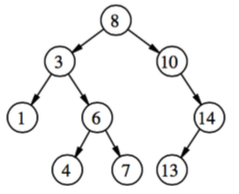
\includegraphics[scale=0.7]{images/binaer}
\centering %centering the image
\caption{Binært tre}
\label{fig:binaer}
\end{figure}

